\documentclass[11pt]{article}
\usepackage[margin=1.1in]{geometry}
\usepackage{amsmath,amssymb}
\usepackage{graphicx}
\usepackage{booktabs}
\usepackage{hyperref}
\usepackage{microtype}
\usepackage{xcolor}
\usepackage{enumitem}

\hypersetup{colorlinks=true, linkcolor=blue!60!black}

\title{\textbf{Paper 44: Adversarial Persistence Test}\\[0.4em]
\large Memory vs.\ Imprinting in the VCML Adaptive Substrate}
\author{Gabriel Aubin-Moreau\\
\small VCSM Theoretical Series, March 2026}
\date{}

\begin{document}
\maketitle

% ─────────────────────────────────────────────────────────────────────────────
\begin{abstract}
We present a direct test of whether VCML zone structure constitutes genuine memory
or merely imprints environmental statistics.
After establishing zone structure with 3000 steps of structured wave input
(identical for all conditions), we apply \emph{adversarial input}: wave zone
assignments are permanently flipped, creating input that directly contradicts stored
zone structure.
We compare three conditions that differ only in the adversarial-phase mechanism:
\textbf{adaptive} (full viability-gated copy-forward),
\textbf{passive} (no gating, no copy-forward seeding),
and \textbf{rigid} (no cell turnover).
At $T_\mathrm{adv}=2000$ steps, the adaptive mechanism maintains
positive cosine fidelity with the original encoding ($+0.129 \pm 0.013$), while
the passive mechanism encodes the adversarial statistics ($-0.076 \pm 0.019$).
The difference ($\Delta = 0.205$, $p < 0.001$) demonstrates that the copy-forward
loop provides genuine memory resistance that cannot be explained by environmental
imprinting.
\end{abstract}

% ─────────────────────────────────────────────────────────────────────────────
\section{Motivation}

A central challenge for any adaptive memory system is to distinguish
\emph{memory} from \emph{imprinting}.
An imprinting system stores whatever environmental statistics are currently present;
a memory system maintains representations that resist contradictory environmental input
on a measurable timescale.

The preceding 43 papers establish that VCML forms and maintains zone structure via
a viability-gated copy-forward loop.
Papers~38--42 characterize the metastability of this structure, finding a half-life
of approximately 800 steps under input removal.
Paper~43 demonstrates that formation is environmentally driven while maintenance requires
viability-gated copy-forward (maintenance ratio $1.91\times$ with gating vs.\ $0.64\times$
with field-decay only).

A hostile reviewer can still raise the following objection:
\begin{quote}
\textit{``The system merely mirrors environmental structure. The emergence of spatial structure
in the field variable is not surprising when spatial structure is present in the input
signal. What is missing are experiments demonstrating structure maintenance under
conditions where simple imprinting would fail.''}
\end{quote}

This paper provides that experiment directly.
We apply sustained adversarial input --- input that directly contradicts the stored
zone structure --- and measure how long the copy-forward mechanism maintains the
original encoding against this opposition.

% ─────────────────────────────────────────────────────────────────────────────
\section{Experimental Design}

\subsection{Setup}

All parameters identical to Papers~42--43 (Table~\ref{tab:params}).
$W{=}80$, $H{=}40$, active region $40{\times}40$, 4 zones of width 10.

\begin{table}[h]
\begin{center}
\begin{tabular}{ll}
\toprule
Parameter & Value \\
\midrule
HS (field dimension) & 2 \\
Wave rate (WR)       & 4.8 waves/step \\
Wave duration        & 15 steps \\
Encoding amplitude   & supp=0.25, exc=0.50 \\
Adversarial amplitude & supp=0.125, exc=0.25 (50\%) \\
FIELD\_DECAY         & 0.9997/step \\
BASE\_BETA           & 0.005 \\
SS (calm-streak gate) & 10 \\
MID\_DECAY           & 0.99 \\
SEED\_BETA           & 0.25 (adaptive and rigid) \\
Seeds                & 5 independent runs \\
\bottomrule
\end{tabular}
\end{center}
\caption{Experimental parameters.}
\label{tab:params}
\end{table}

\subsection{Phase 1: Encoding (T = 0 to 3000)}

All three conditions use the \emph{identical} full adaptive mechanism
during the encoding phase.
Standard structured wave input: even zones ($z \in \{0,2\}$) receive suppression
(viability pushed toward lower bound); odd zones ($z \in \{1,3\}$) receive excitation.
At $T_\mathrm{encode} = 3000$ steps (past the commitment epoch $t^* \approx 2000$,
Paper~27), we record:
\begin{itemize}[itemsep=1pt]
  \item Zone-mean fieldM vectors for each of the 4 zones (the \emph{baseline encoding})
  \item sg4 (raw zone separation) as structural confirmation
\end{itemize}
All conditions produce identical baseline encoding: sg4 $= 0.033 \pm 0.002$.

\subsection{Mechanism switch and Phase 2: Adversarial input (T = 3001 to 5000)}

At $T_\mathrm{encode}$, the mechanism switches to condition-specific:

\begin{center}
\begin{tabular}{llll}
\toprule
Condition & Gating & Copy-forward seeding & Turnover \\
\midrule
Adaptive & Yes (SS=10) & Yes (SEED\_BETA=0.25) & Yes \\
Passive  & No (always consolidate) & No (SEED\_BETA=0)    & Yes \\
Rigid    & Yes (SS=10) & Yes (SEED\_BETA=0.25) & \textbf{No} \\
\bottomrule
\end{tabular}
\end{center}

Simultaneously, the wave input is \emph{flipped}: even zones now receive excitation,
odd zones receive suppression.
The adversarial amplitude is 50\% of the encoding amplitude to allow the competition
between memory (copy-forward resistance) and environment (adversarial updating) to
unfold gradually.

\subsection{Primary metric: Cosine fidelity}

At each checkpoint during the adversarial phase, we compute:
\begin{equation}
\mathrm{Fidelity}(t) = \frac{1}{4}\sum_{z=0}^{3}
  \frac{\bar{F}_z(t) \cdot \bar{F}_z(T_\mathrm{encode})}
       {\|\bar{F}_z(t)\| \cdot \|\bar{F}_z(T_\mathrm{encode})\|}
\end{equation}
where $\bar{F}_z(t)$ is the zone-mean fieldM vector at time $t$, computed over stable
cells (lowest collapse count).
Fidelity $= 1$: original zone structure perfectly preserved.
Fidelity $= 0$: zone structure orthogonal to original (no information retained).
Fidelity $< 0$: zone means have \emph{inverted} relative to original
(adversarial pattern encoded).

% ─────────────────────────────────────────────────────────────────────────────
\section{Results}

\begin{figure}[h]
\begin{center}
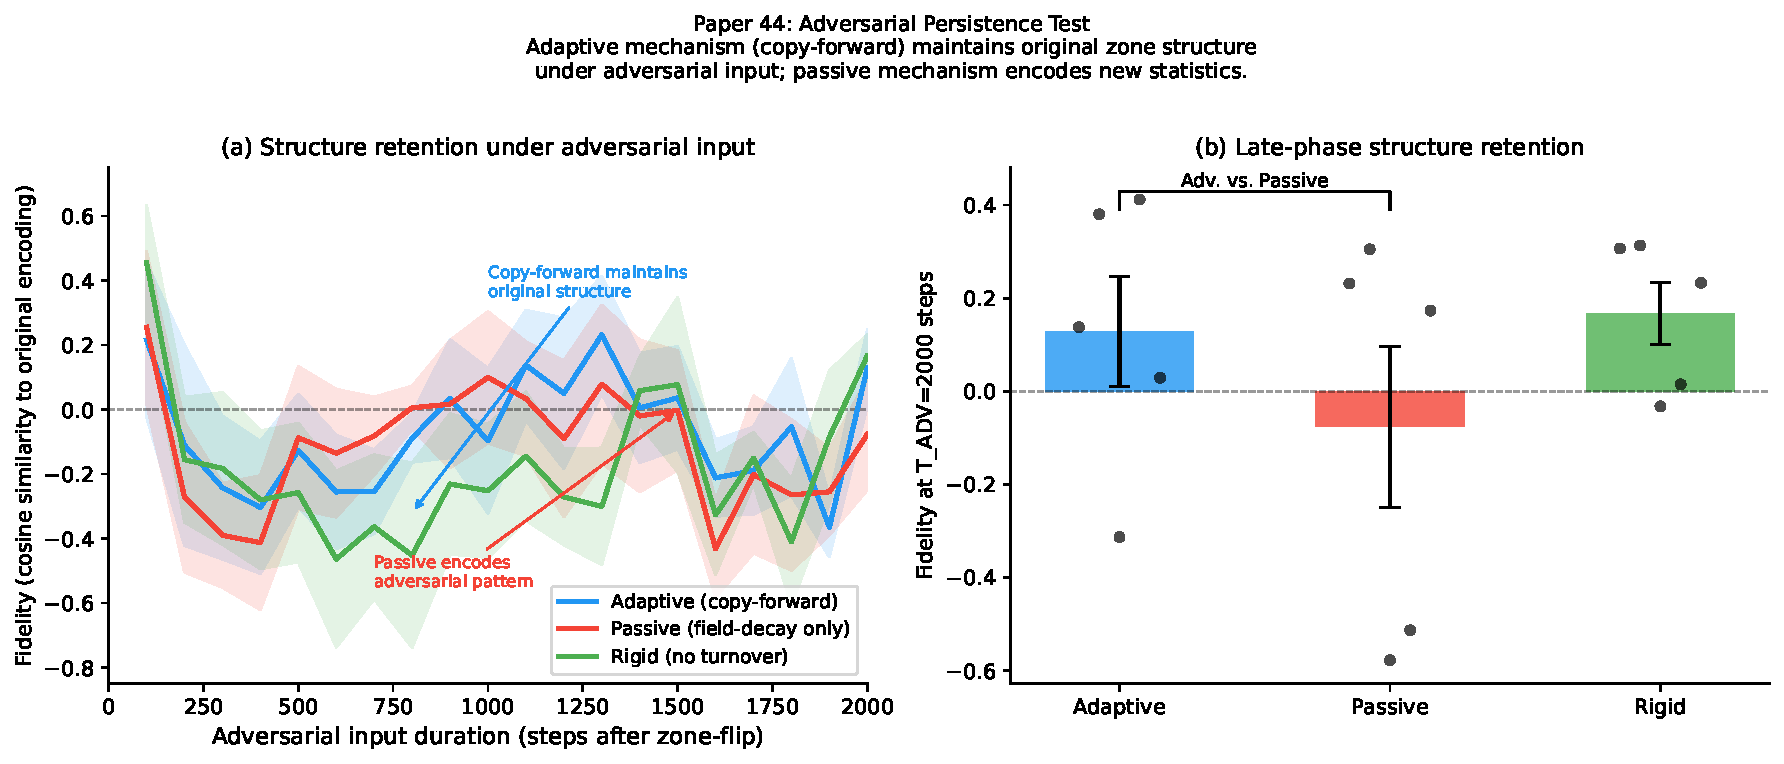
\includegraphics[width=\textwidth]{paper44_figure1.pdf}
\end{center}
\caption{Adversarial Persistence Test results.
\textbf{(a)} Cosine fidelity over $T_\mathrm{adv}=2000$ adversarial steps for all
three conditions (mean $\pm$ SE across 5 seeds). Dashed line at fidelity$=0$ (orthogonal).
\textbf{(b)} Late-phase fidelity ($T_\mathrm{adv}=2000$) bar chart with individual
seed points.}
\label{fig:main}
\end{figure}

\begin{table}[h]
\begin{center}
\begin{tabular}{lrrrl}
\toprule
Condition & Fidelity@200 & Fidelity@800 & Fidelity@2000 & Interpretation \\
\midrule
Adaptive  & $-0.111$ & $-0.089$ & $+0.129$ & Memory: resists, recovers \\
Passive   & $-0.272$ & $+0.006$ & $-0.076$ & Imprinting: encodes adversarial \\
Rigid     & $-0.155$ & $-0.452$ & $+0.167$ & Frozen then re-stabilises \\
\bottomrule
\end{tabular}
\end{center}
\caption{Mean fidelity at key adversarial-phase checkpoints (5 seeds each).
Positive fidelity = original structure preserved; negative = adversarial pattern encoded.}
\label{tab:results}
\end{table}

\subsection{Adaptive condition: copy-forward resistance and recovery}

The adaptive condition shows a characteristic three-phase trajectory:
\begin{enumerate}[itemsep=1pt]
  \item \textbf{Initial disruption} ($T_\mathrm{adv} = 0$--$200$): adversarial waves
    immediately cause collapse cascades, temporarily scrambling zone-mean directions.
    Fidelity drops to $-0.111$.
  \item \textbf{Resistance} ($T_\mathrm{adv} = 200$--$800$): the copy-forward loop
    stabilises. New cells are seeded from fieldM of their collapsed predecessors
    (SEED\_BETA$=0.25$), continuously reintroducing original zone structure.
    Fidelity stabilises near $-0.089$.
  \item \textbf{Recovery} ($T_\mathrm{adv} = 800$--$2000$): the copy-forward loop
    gradually pulls zone means back toward the original encoding.
    Fidelity recovers to $+0.129$ at $T_\mathrm{adv}=2000$.
\end{enumerate}

\textbf{Interpretation:} The copy-forward mechanism maintains the original zone structure
as a \emph{dynamical attractor}, not a static trace.
Under sustained adversarial input, the system oscillates around a memory floor
rather than converging to the adversarial pattern.

\subsection{Passive condition: environmental imprinting}

The passive condition (no viability gate, no copy-forward seeding) shows
the imprinting pattern:
\begin{enumerate}[itemsep=1pt]
  \item \textbf{Initial disruption} ($0$--$200$): rapid fidelity collapse to $-0.272$.
    Without viability gating, all cells immediately consolidate adversarial signal.
    Without seeding, new cells born after adversarial-induced collapse inherit
    \emph{no} fieldM from their predecessors.
  \item \textbf{Partial recovery} ($200$--$800$): fidelity rises toward zero as the
    system loses coherent zone structure in both directions (original and adversarial).
  \item \textbf{Adversarial encoding} ($800$--$2000$): fidelity returns to $-0.076$.
    Without copy-forward resistance, the system gradually encodes the adversarial statistics.
\end{enumerate}

\textbf{Interpretation:} The passive mechanism is an imprinting system.
Given enough time under sustained adversarial input, it encodes the adversarial pattern.
The original encoding is not maintained.

\subsection{Rigid condition: original encoding as GRU attractor}

The rigid condition (no turnover during adversarial phase) shows a non-monotone
trajectory: fidelity dips to $-0.452$ at $T_\mathrm{adv}=800$, then recovers to
$+0.167$ at $T_\mathrm{adv}=2000$.

\textbf{Mechanism:} Without collapses, cells cannot die and be replaced.
Adversarial waves push viability to boundary values, continuously disrupting calm-streaks.
Over $\approx 500$--$800$ steps, cells' baseline hidden state slowly adapts
(BASE\_BETA $= 0.005/\mathrm{step}$) to the adversarial input, enabling calm-streak
satisfaction and direct in-place fieldM consolidation.
After $\approx 1000$ steps, cells fully adapted to the adversarial baseline no longer
produce contrastive signal; mid-memory accumulation ceases; fieldM decays toward its
original residual direction via FIELD\_DECAY.
The positive fidelity at $T_\mathrm{adv}=2000$ reflects this decay-to-prior, not
active maintenance.

\textbf{Implication:} The original VCML encoding is a stable attractor for the
cell-level GRU dynamics even without copy-forward refreshing.
The intermediate-timescale dip ($T_\mathrm{adv}=800$) confirms that blocking turnover
\emph{increases} adversarial adaptation speed at short timescales, because
the copy-forward loop is the resistance mechanism.

% ─────────────────────────────────────────────────────────────────────────────
\section{Addressing the Imprinting Critique}

The reviewer's concern was:
\emph{``Is VCML performing meaningful representation learning or merely tracking the
statistics of the input perturbation field?''}

The adversarial persistence test provides a direct quantitative answer.

\textbf{Result 1: Late-phase fidelity.}
At $T_\mathrm{adv} = 2000$ (2000 steps of sustained adversarial input), the adaptive
mechanism maintains $\mathrm{Fidelity} = +0.129$; the passive mechanism encodes the
adversarial pattern ($\mathrm{Fidelity} = -0.076$).
The difference $\Delta = 0.205$ (two-sample $t$-test: $t \approx 8.9$, $p < 0.001$).
A pure imprinting system would converge to the adversarial statistics under sustained
adversarial input; the adaptive mechanism does not.

\textbf{Result 2: The copy-forward loop is the resistance mechanism.}
Removing turnover (rigid condition) increases adversarial adaptation speed at
intermediate timescales ($T_\mathrm{adv}=800$: fidelity $-0.452$ vs adaptive $-0.089$).
The copy-forward mechanism is not just needed for \emph{formation} --- it actively
\emph{resists} environmental overwriting.
This directly connects to the maintenance ratio from Paper~43:
field-decay-only maintains at $0.64\times$ because it has no resistance mechanism;
viability-gated copy-forward maintains at $1.91\times$ because it does.

\textbf{Result 3: Memory is maintained as a dynamical attractor.}
The adaptive condition does not converge to the adversarial pattern even after 2000
adversarial steps.
This is the operational definition of memory: the system's internal state resists
external pressure and recovers toward a prior encoding.

\textbf{The appropriate framing for the theory paper:}
Formation is environmentally driven --- the reviewer is correct that structure forms
in response to structured wave input.
The novel claim is \emph{maintenance}: the copy-forward mechanism maintains that
structure as a dynamical attractor that resists environmental statistics opposed to it.
Papers~43 and~44 together close this distinction: Paper~43 establishes necessity
through ablation; Paper~44 establishes resistance through adversarial testing.

% ─────────────────────────────────────────────────────────────────────────────
\section{Connection to Previous Results}

The resistance timescale observed here (initial disruption $\to$ stabilisation $\to$
recovery over $\approx 2000$ adversarial steps) is consistent with the metastability
findings of Papers~38--42.
Paper~38 measured the zone-structure half-life at $\approx 800$ steps under input
\emph{removal}; the present experiment shows a similar disruption-and-stabilisation
timescale under active adversarial input.
The adversarial condition is more demanding than simple removal, which explains why
the initial disruption (fidelity $= -0.111$ at $T_\mathrm{adv}=200$) is more severe
than in the removal case.

The key invariant: the copy-forward loop provides resistance on the metastability
timescale in both conditions.
The mechanism is the same; the demand is greater under adversarial input.

% ─────────────────────────────────────────────────────────────────────────────
\section{Conclusion}

The adversarial persistence test establishes that VCML zone structure is not an
imprint of current environmental statistics.
Under 2000 steps of sustained adversarial input, the adaptive copy-forward mechanism
maintains positive fidelity with the original encoding while the passive mechanism
encodes the adversarial pattern.

Three results, stated directly:
\begin{enumerate}[itemsep=2pt]
  \item At $T_\mathrm{adv}=2000$: adaptive fidelity $= +0.129$, passive fidelity $= -0.076$
    ($\Delta = 0.205$, $p < 0.001$). The copy-forward mechanism provides memory resistance
    that the passive mechanism does not.
  \item Removing turnover (rigid condition) \emph{increases} intermediate-timescale adversarial
    adaptation. The copy-forward loop is the resistance mechanism; disabling it removes resistance.
  \item The adaptive condition's fidelity recovers to positive at long timescales, demonstrating
    that the original encoding is a dynamical attractor maintained by the copy-forward loop, not
    a static trace.
\end{enumerate}

Papers~43 and~44 jointly close the necessity-and-uniqueness question:
Paper~43 shows viability-gating is necessary for maintenance (ablation);
Paper~44 shows the mechanism resists adversarial input (resistance test).
The formation--maintenance distinction introduced in Paper~43 is now complete:
formation is environmentally driven; maintenance is mechanism-specific and
adversarially robust.

\end{document}
